\documentclass[12pt]{article}

% Based upon https://tikz.dev/library-er

\usepackage{tikz}
\usetikzlibrary{er,positioning} 

\begin{document}
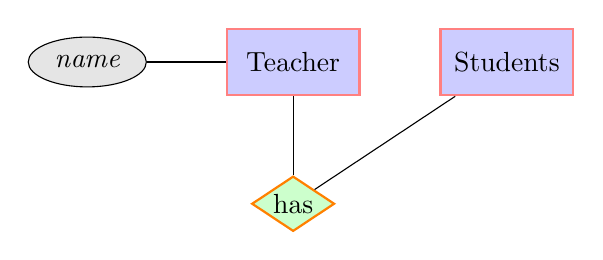
\begin{tikzpicture}
    [every entity/.style={draw=red!50,fill=blue!20,thick},
    every relationship/.style={fill=green!20,draw=orange,thick,aspect=1.5},
    every attribute/.style={fill=gray!20,draw=black}]

    \node[entity] (Teacher) {Teacher} child {node  [key attribute] [left=of Teacher] {name}};
    \node[entity] (Students) [right=of Teacher] {Students};
    \node[relationship] [below=of Teacher] {has} edge (Teacher) edge (Students);
\end{tikzpicture}
\end{document}